\documentclass[tikz,border=3pt]{standalone}
\usepackage[utf8]{inputenc}
\usepackage[T1]{fontenc}
\usepackage{lmodern}
\renewcommand{\familydefault}{\sfdefault}
\usepackage{sansmath}\sansmath
\usepackage{pgfplots}\pgfplotsset{compat=1.18,/pgf/number format/use comma,/pgf/number format/1000 sep={.}}
\usetikzlibrary{arrows.meta,calc,positioning,decorations.pathmorphing,patterns}
% paleta del sitio
\definecolor{nar}{HTML}{E8680C}\definecolor{narc}{HTML}{FFB35C}\definecolor{hielo}{HTML}{FFF3E8}
\definecolor{tinta}{HTML}{1D1D1F}\definecolor{gris}{HTML}{6E6E73}\definecolor{lila}{HTML}{7C5CF0}
\definecolor{azul}{HTML}{2F6FD6}\definecolor{menta}{HTML}{17A673}\definecolor{coral}{HTML}{E8342A}
\begin{document}
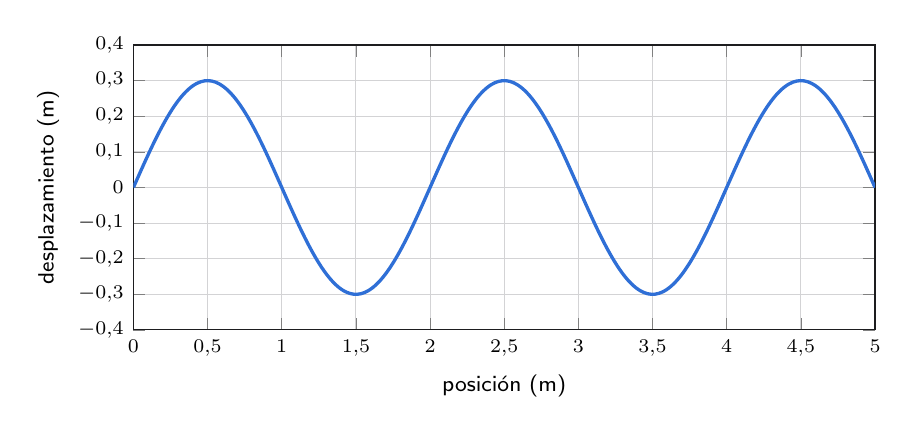
\begin{tikzpicture}[font=\footnotesize,>={Stealth[length=2.4mm]}]
\begin{axis}[width=11cm,height=5.2cm,xmin=0,xmax=5,ymin=-0.4,ymax=0.4,
  xtick={0,0.5,...,5},ytick={-0.4,-0.3,-0.2,-0.1,0,0.1,0.2,0.3,0.4},
  yticklabel style={/pgf/number format/fixed,/pgf/number format/precision=1},
  grid=both,grid style={gris!30},axis line style={tinta},
  xlabel={posición (m)},ylabel={desplazamiento (m)},tick label style={font=\scriptsize}]
\addplot[very thick,azul,domain=0:5,samples=200,smooth] {0.3*sin(180*x)};
\end{axis}
\end{tikzpicture}
\end{document}
